% Options for packages loaded elsewhere
\PassOptionsToPackage{unicode}{hyperref}
\PassOptionsToPackage{hyphens}{url}
%
\documentclass[
]{article}
\usepackage{amsmath,amssymb}
\usepackage{lmodern}
\usepackage{iftex}
\ifPDFTeX
  \usepackage[T1]{fontenc}
  \usepackage[utf8]{inputenc}
  \usepackage{textcomp} % provide euro and other symbols
\else % if luatex or xetex
  \usepackage{unicode-math}
  \defaultfontfeatures{Scale=MatchLowercase}
  \defaultfontfeatures[\rmfamily]{Ligatures=TeX,Scale=1}
\fi
% Use upquote if available, for straight quotes in verbatim environments
\IfFileExists{upquote.sty}{\usepackage{upquote}}{}
\IfFileExists{microtype.sty}{% use microtype if available
  \usepackage[]{microtype}
  \UseMicrotypeSet[protrusion]{basicmath} % disable protrusion for tt fonts
}{}
\makeatletter
\@ifundefined{KOMAClassName}{% if non-KOMA class
  \IfFileExists{parskip.sty}{%
    \usepackage{parskip}
  }{% else
    \setlength{\parindent}{0pt}
    \setlength{\parskip}{6pt plus 2pt minus 1pt}}
}{% if KOMA class
  \KOMAoptions{parskip=half}}
\makeatother
\usepackage{xcolor}
\usepackage[margin=1in]{geometry}
\usepackage{graphicx}
\makeatletter
\def\maxwidth{\ifdim\Gin@nat@width>\linewidth\linewidth\else\Gin@nat@width\fi}
\def\maxheight{\ifdim\Gin@nat@height>\textheight\textheight\else\Gin@nat@height\fi}
\makeatother
% Scale images if necessary, so that they will not overflow the page
% margins by default, and it is still possible to overwrite the defaults
% using explicit options in \includegraphics[width, height, ...]{}
\setkeys{Gin}{width=\maxwidth,height=\maxheight,keepaspectratio}
% Set default figure placement to htbp
\makeatletter
\def\fps@figure{htbp}
\makeatother
\setlength{\emergencystretch}{3em} % prevent overfull lines
\providecommand{\tightlist}{%
  \setlength{\itemsep}{0pt}\setlength{\parskip}{0pt}}
\setcounter{secnumdepth}{-\maxdimen} % remove section numbering
\ifLuaTeX
  \usepackage{selnolig}  % disable illegal ligatures
\fi
\IfFileExists{bookmark.sty}{\usepackage{bookmark}}{\usepackage{hyperref}}
\IfFileExists{xurl.sty}{\usepackage{xurl}}{} % add URL line breaks if available
\urlstyle{same} % disable monospaced font for URLs
\hypersetup{
  pdftitle={Measuring Term Premia for the Euro Area},
  hidelinks,
  pdfcreator={LaTeX via pandoc}}

\title{Measuring Term Premia for the Euro Area}
\author{}
\date{\vspace{-2.5em}Dev Prakash Srivastava}

\begin{document}
\maketitle

\bigskip\bigskip

\textbf{INTRODUCTION}

This project aims to compute estimates of term premia for the Euro Area
- specifically for the countries Germany, France, Spain and Italy. We
will first give empirical estimates for the term premia for the
historical series beginning from 2000 to the present. For that we use
two approaches - predictive model and consensus forecast (will be
explained later). The aim is to estimate the term premia for the present
long term Euro area bonds, and also to allow the user to enter the
suitable parameters/forecasts to obtain the term premia.

The report gives the procedure used for the computation of the estimates
and summarize the results obtained.

\bigskip\bigskip

\textbf{THEORETICAL FRAMEWORK}

We first underline the theoretical framework used.

Consider zero-coupon bonds and apply the no arbitrage condition to a
one-period bond (the safe asset) and a T-period bond:

\[ E_{t}( r_{t,t+1}^{T}-r_{t,t+1}^{1}) = E_{t}(
        r_{t,t+1}^{T}-y_{t,t+1}) =\phi _{t,t+1}^{T} \\
        E_{t}( r_{t,t+1}^{T}) = y_{t,t+1}+\phi _{t,t+1}^{T} \]

Solving forward the difference equation
\(p_{t,T}=p_{t+1,T}-r_{t,t+1}^{T},\) we have :

\begin{eqnarray*}
        y_{t,T} &=&\frac{1}{\left( T-t\right) }\underset{i=0}{\overset{T-1}{\sum }}%
        E_{t}\left( r_{t+i,t+i+1}^{T}\right) \\
        &=&\frac{1}{\left( T-t\right) }\underset{i=0}{\overset{T-1}{\sum }}%
        E_{t}\left( y_{t+i,t+i+1}+\phi _{t+i,t+i+1}^{T}\right)
\end{eqnarray*} So we have the following equation for the term spread
\begin{eqnarray*}
    y_{t,T}-y_{t,t+1}= \underset{i=1}{\overset{T-t-1}{\sum}}\left(1-\frac{i}{T-t}\right)E_{t}\Delta y_{t+i,t+i+1}+\frac{1}{T-t}\underset{i=1}{\overset{T-t-1}{\sum }}\phi _{t+i,t+i+1}^{T}
\end{eqnarray*}

\bigskip

\textbf{PROCEDURE}

We can use the term spread equation given above to estimate the term
premia. We use the common short-rate for the Euro Area, and the yields
on the 10-year government bond yields for the term spread. But the
future expected future path of short-term rates is not known and thus we
need some approach to estimate \(\Delta y_{t+i,t+i+1}\). Once we have
it, the term premia can be easily calculated.

To estimate the future path of short-term rates we use two approaches -

\begin{enumerate}
\def\labelenumi{\arabic{enumi}.}
\item
  Predictive Model -
  \[ \Delta y_{t+1,t+2} = \rho\Delta y_{t,t+1} + \epsilon_{t+1} \] We
  can estimate \(\rho\) using the historical data available. This
  parameter (assuming it be constant over time) can be used to get the
  future path of interest rates.While basic it can serve as an excellent
  baseline model.
\item
  Consensus forecasts -\\
  The ECB's Professional Forecasters Survey gives the average forecasts
  for the expected future short-term rates. These can be directly used
  and compared with our baseline model estimates.
\end{enumerate}

\bigskip

\textbf{RESULTS}

The following plot compares the long-term bond yields of Germany,
France, Italy and Spain

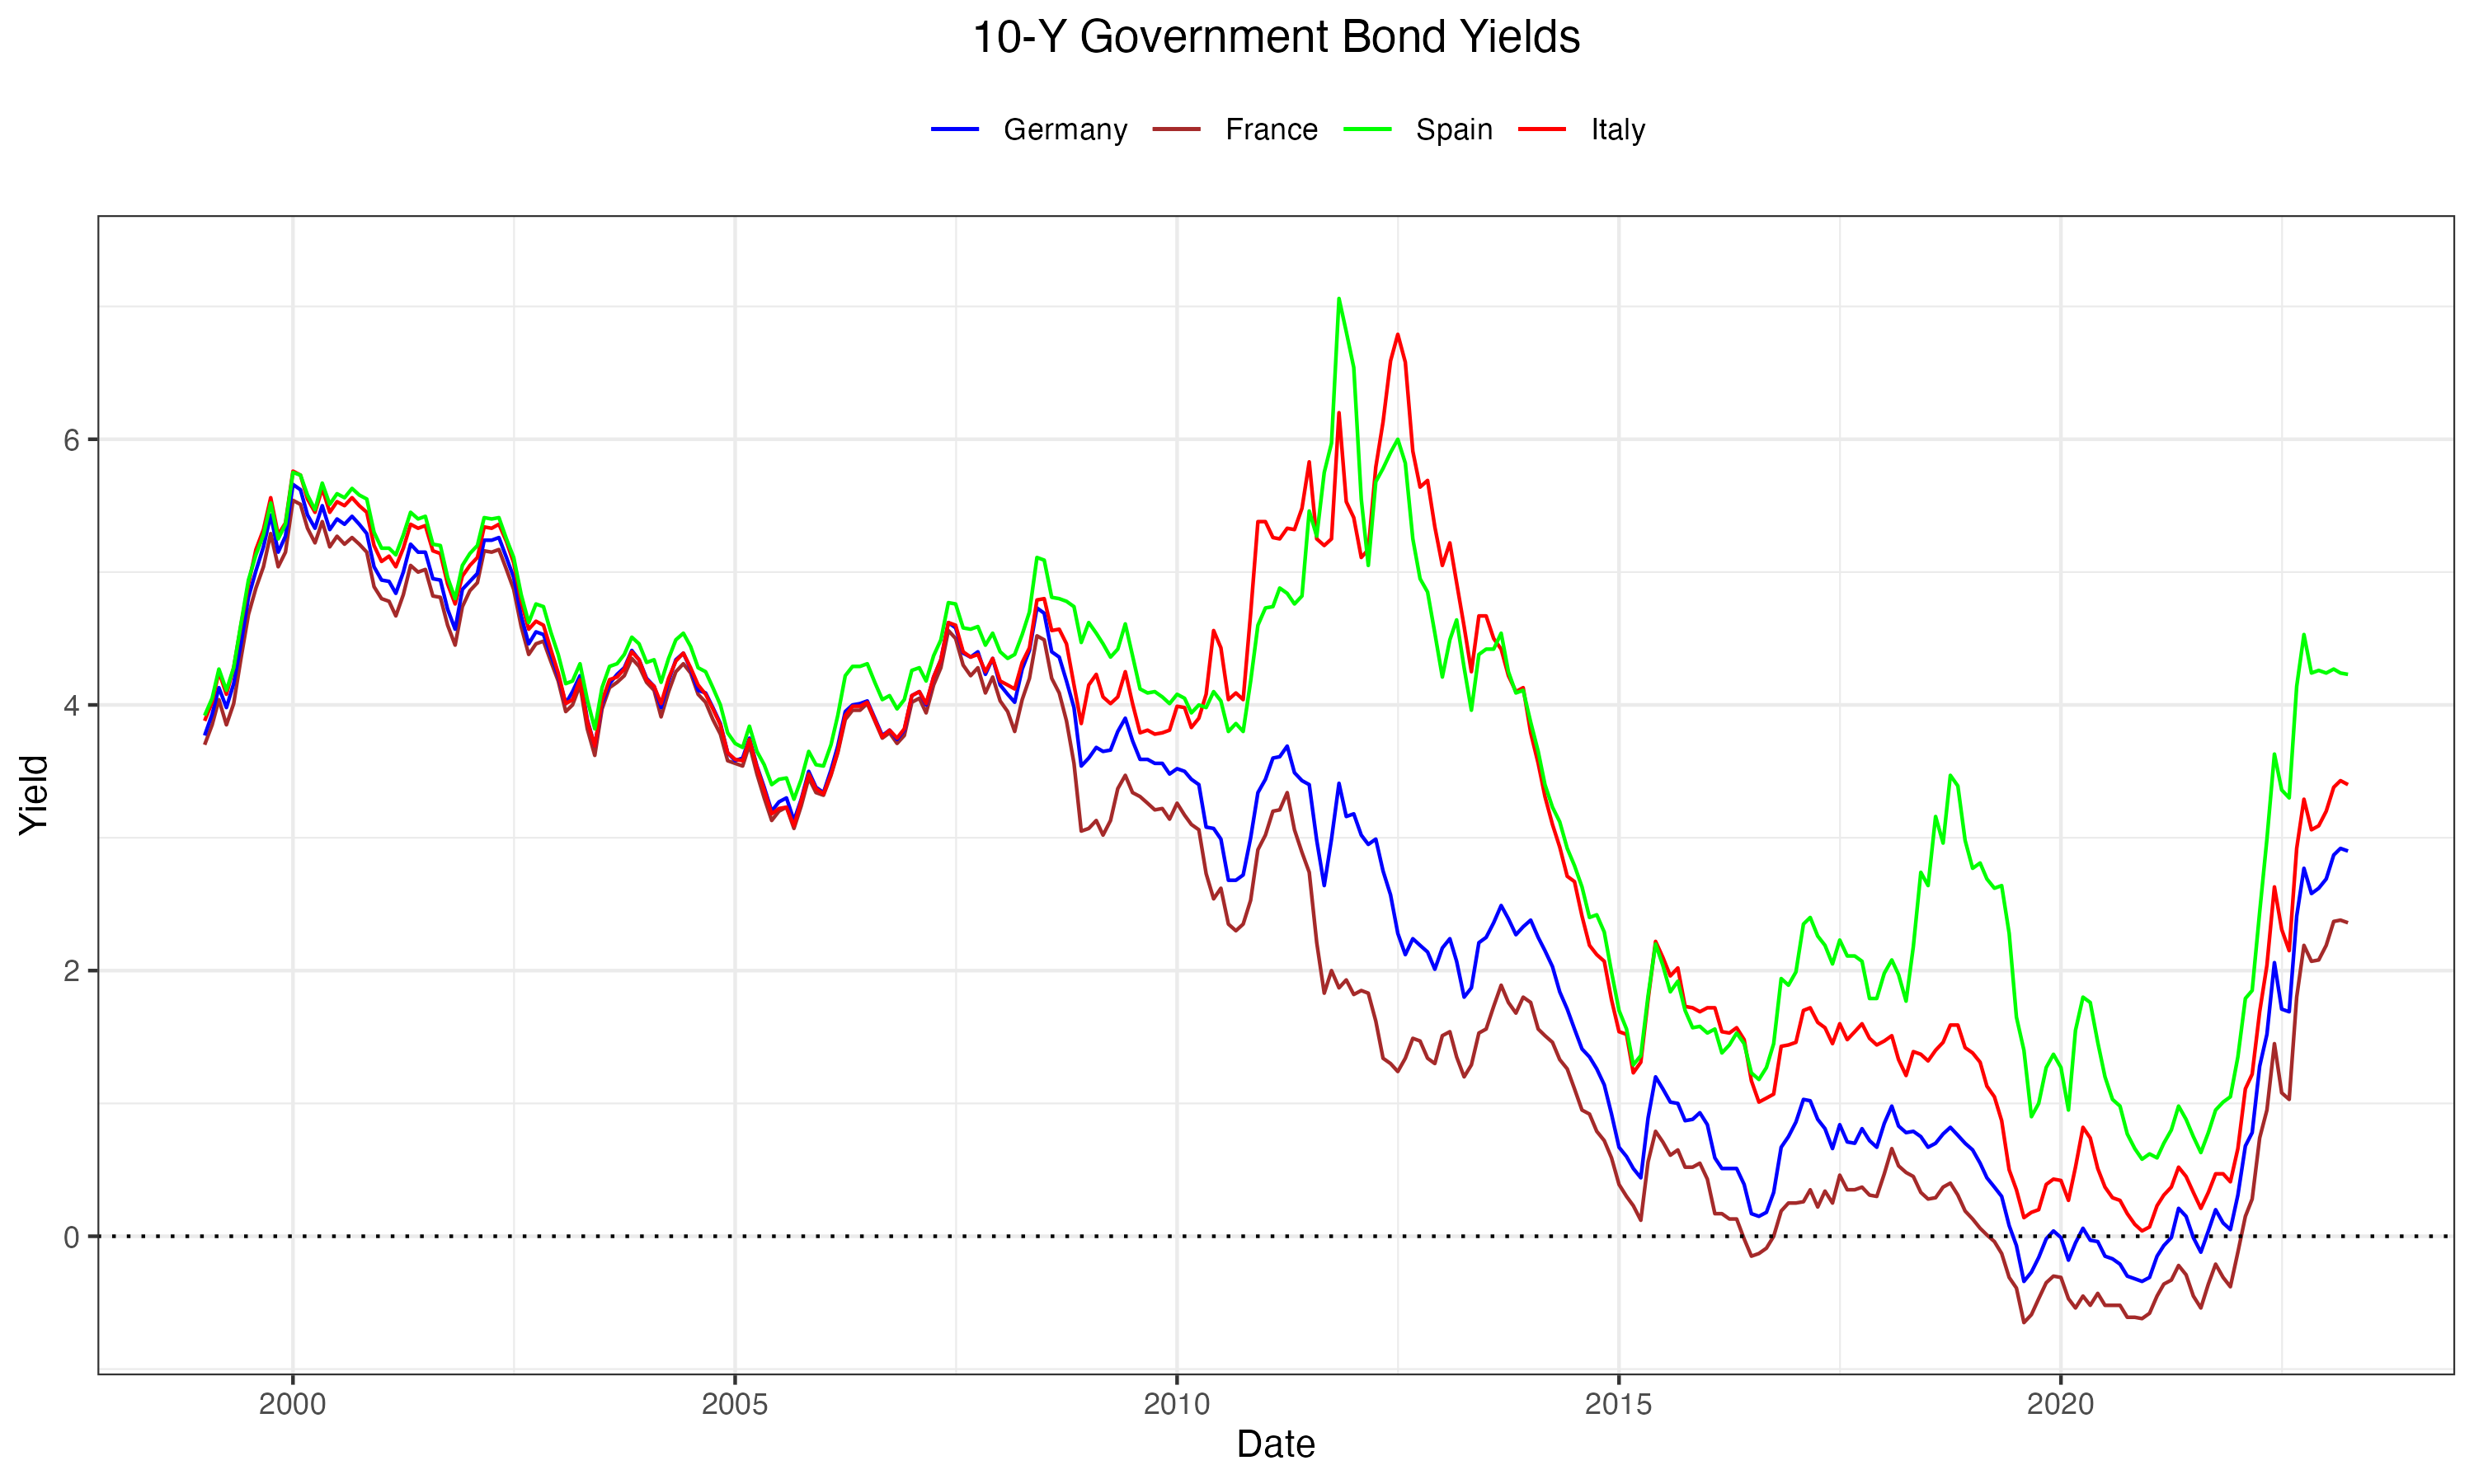
\includegraphics[width=0.8\textwidth,height=\textheight]{Plots/Historical/Long Term Government Bond Yields.png}
\bigskip

We can see one crucial feature - the bond yield were similar across all
the countrie till 2008 and then diverged, with Italy and Spain having
higher long-term-bond yields than Germany and France.

We can also get the yield decompositions for the countries - the term
premia are calculated using the two methods described previously.

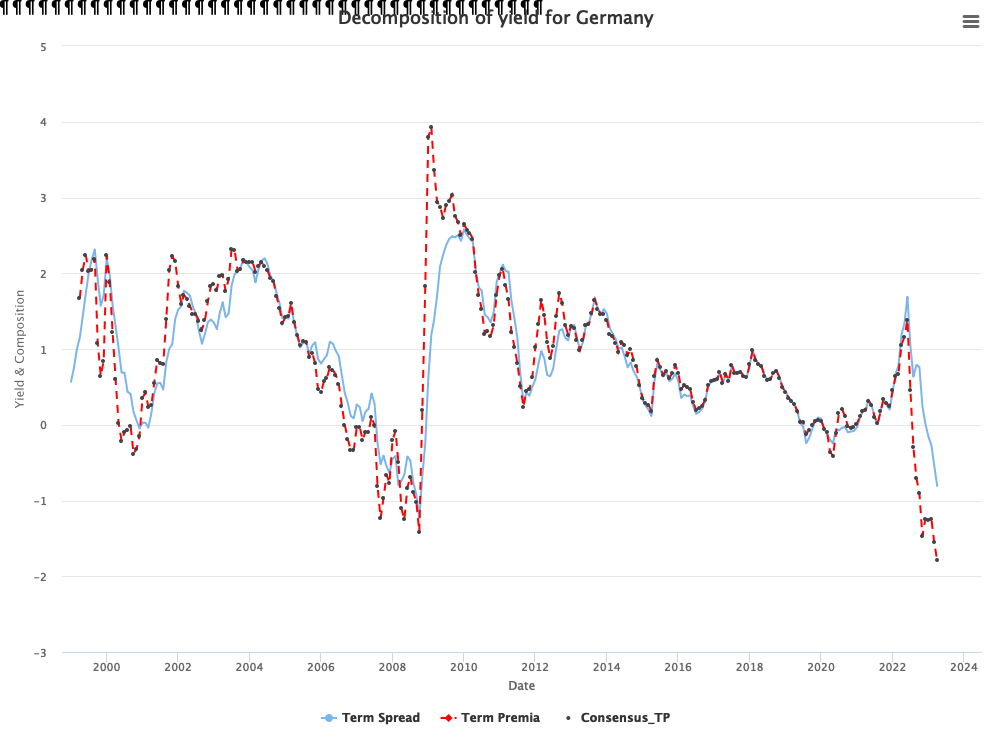
\includegraphics[width=0.5\textwidth,height=\textheight]{Plots/Historical/Yield_decomposition_Germany.png}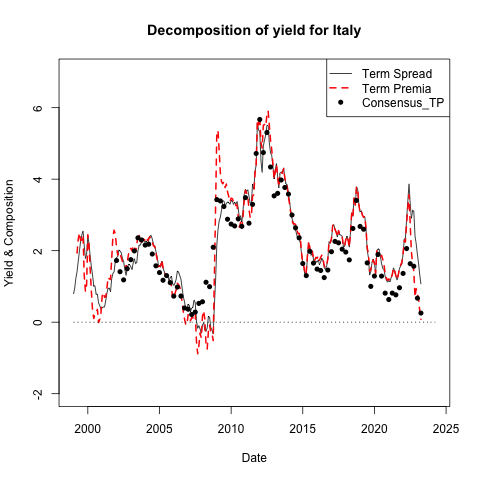
\includegraphics[width=0.5\textwidth,height=\textheight]{Plots/Historical/Yield_decomposition_Italy.png}
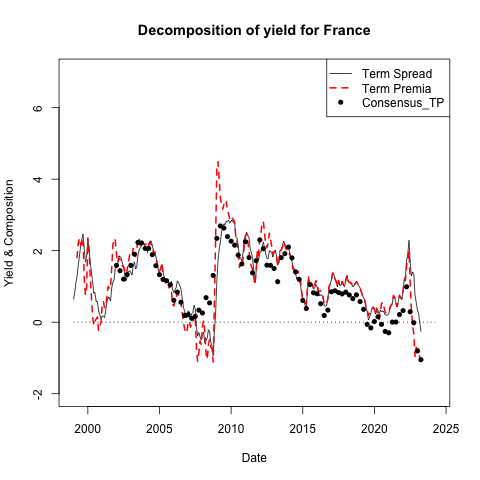
\includegraphics[width=0.5\textwidth,height=\textheight]{Plots/Historical/Yield_decomposition_France.png}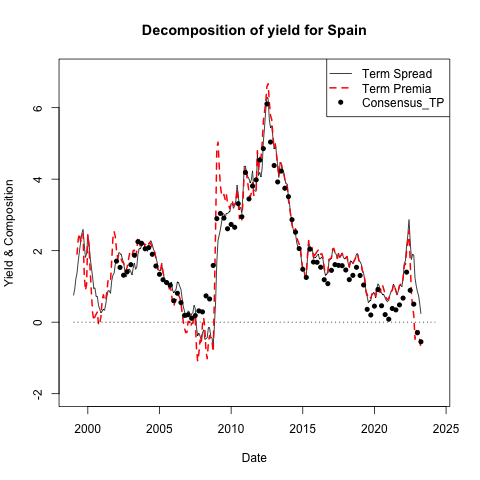
\includegraphics[width=0.5\textwidth,height=\textheight]{Plots/Historical/Yield_decomposition_Spain.png}

From the decomposition plots, we can infer that most of the term spread
can be explained by the term premia, and the short-rate movements
contribute little to the term spread. This has important implications
for\ldots{}

We also see a downward shift of the term premia in the recent years,
with it reaching negative values in Germany and Franc. In Germany, the
term premia has been negative since before even 2020. This matches the
US experience, showing similarities in term premia across the two
regions. \pagebreak

Finally, the following two figures summarise the term premia estimates:

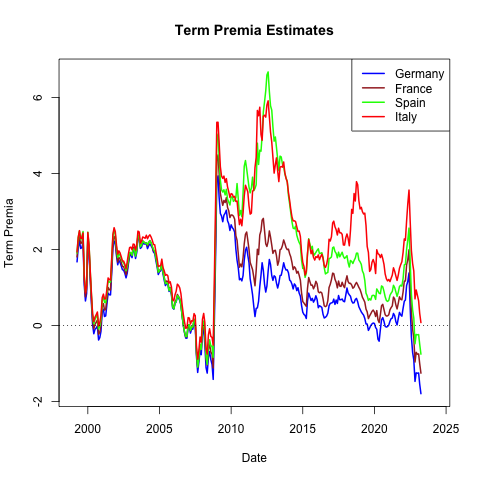
\includegraphics[width=0.5\textwidth,height=\textheight]{Plots/Historical/Model Term Premia estimates.png}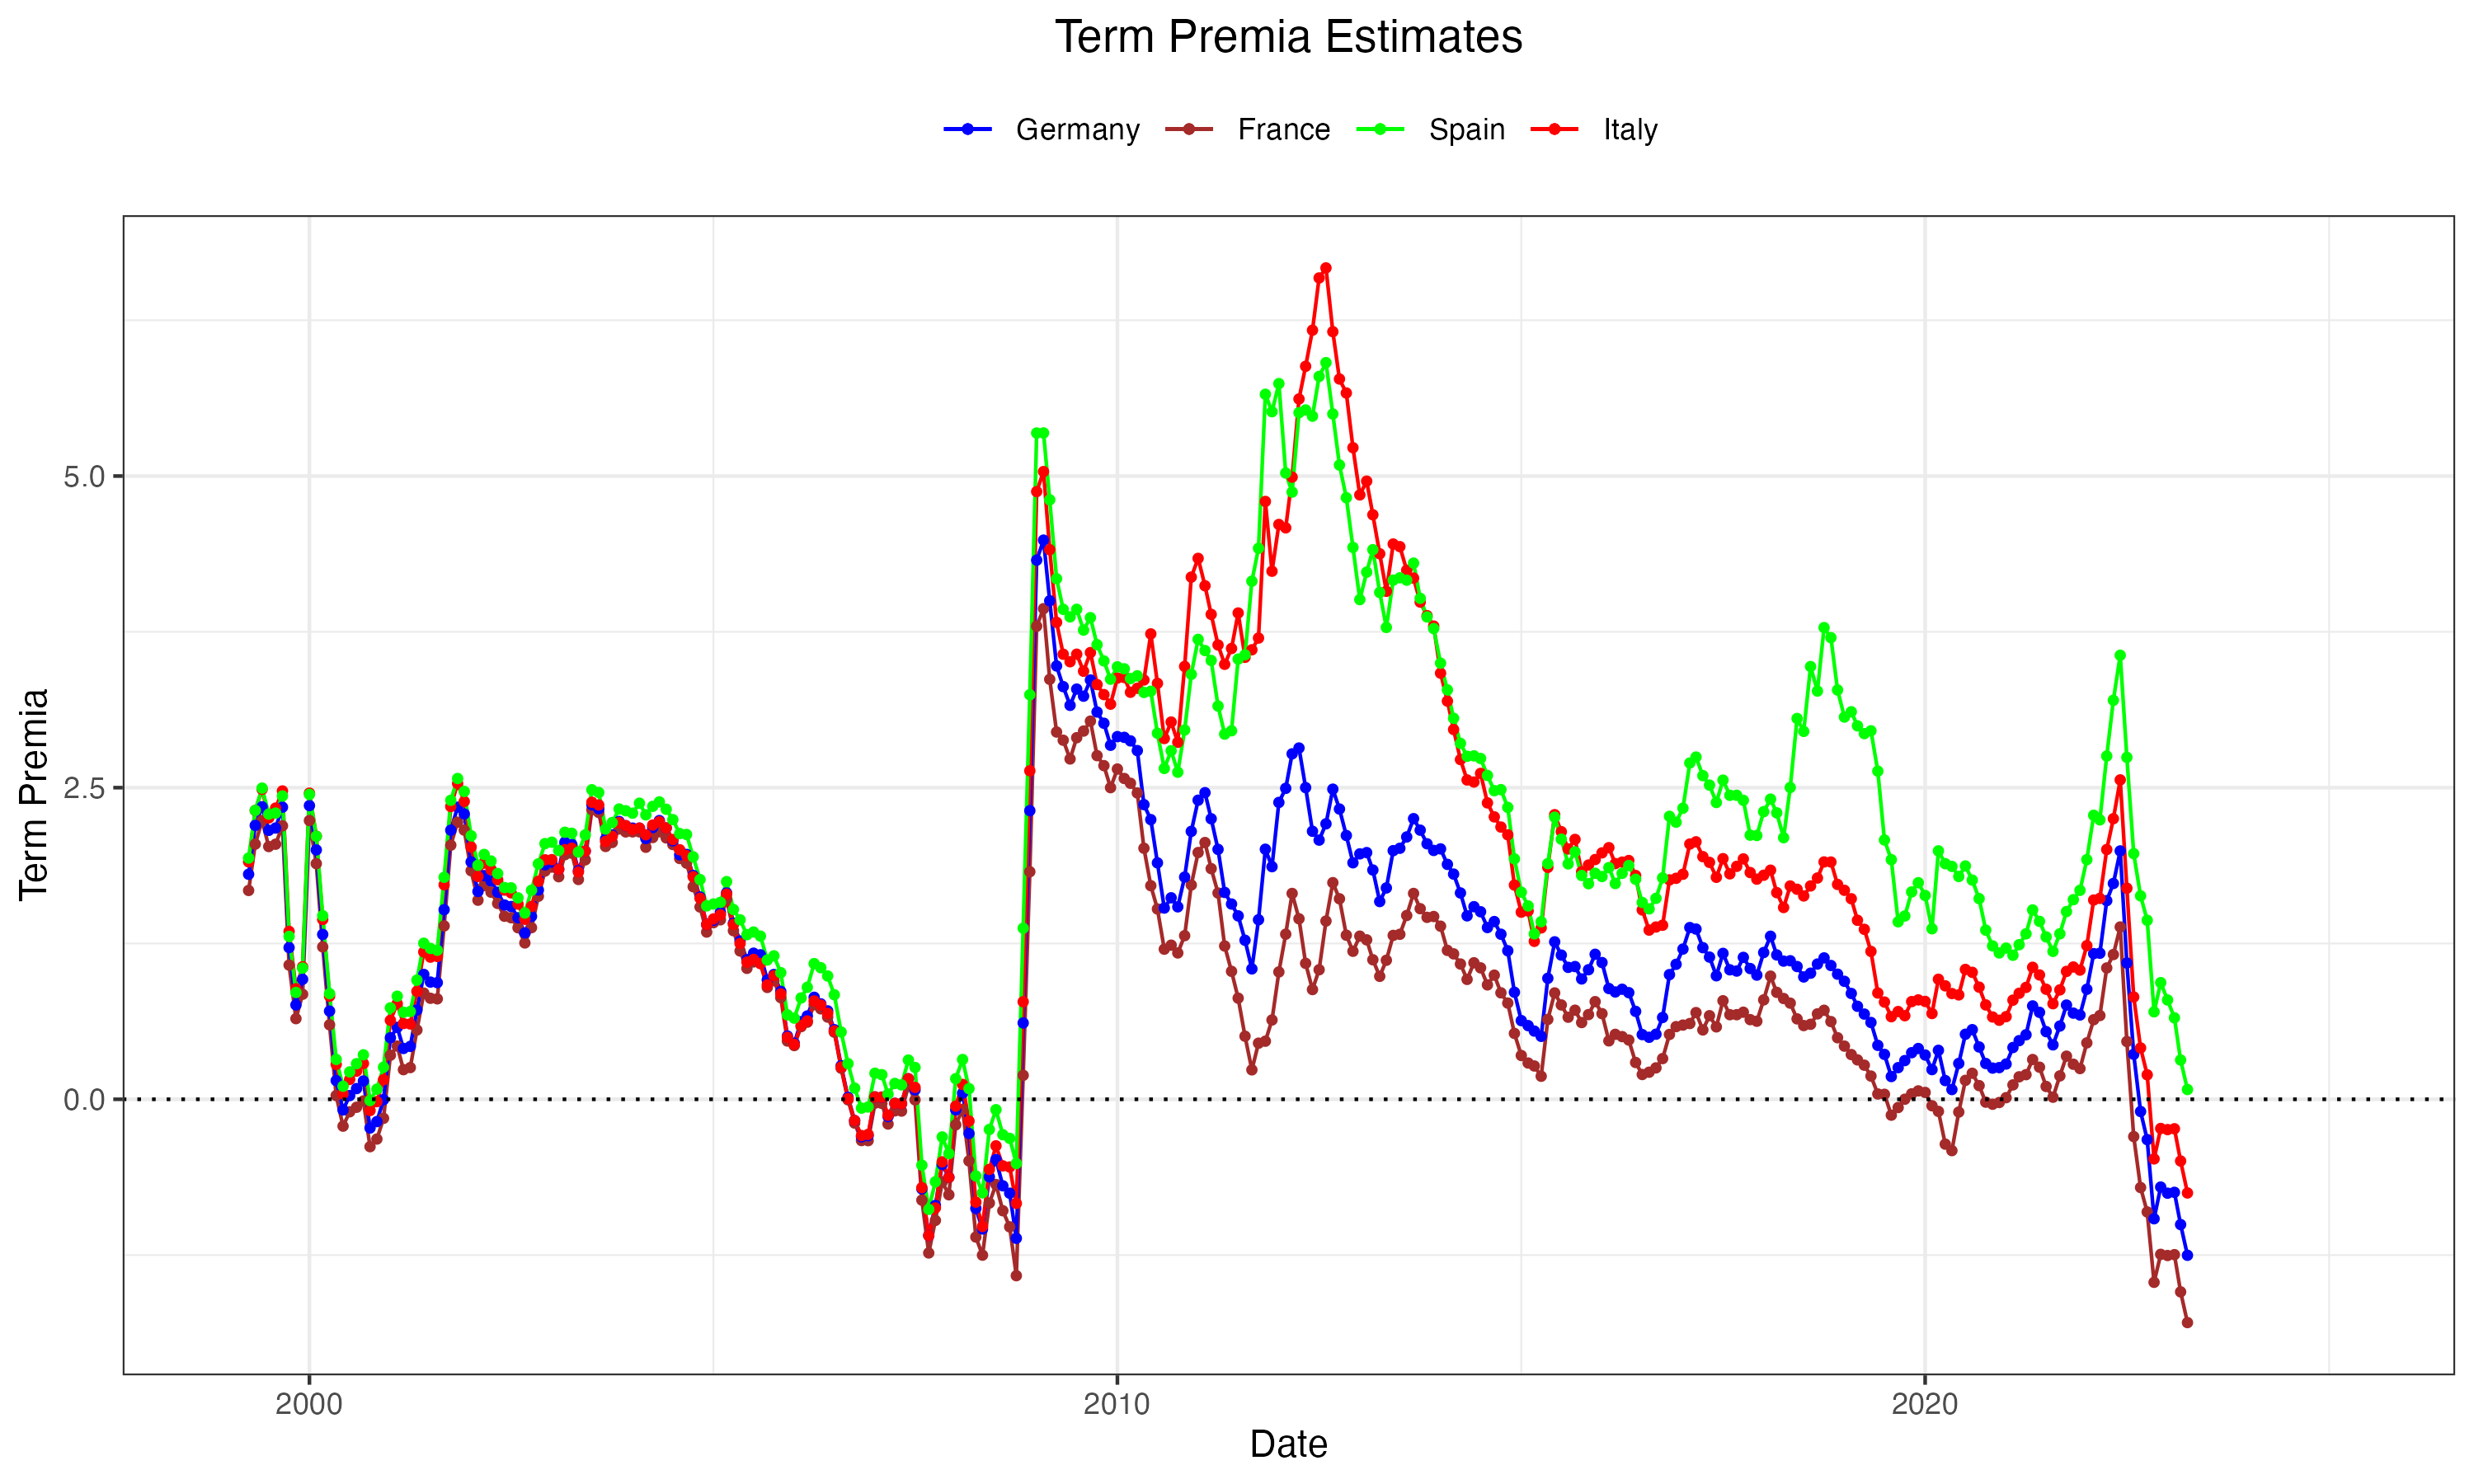
\includegraphics[width=0.5\textwidth,height=\textheight]{Plots/Historical/Consensus Term Premia estimates.png}

\end{document}
